% \respto{2-22}{\color{blue}Given a group of software projects,
% there often exists  one   exemplar project
% that offers the best prediction for all others.
% Such ``bellwether projects''
% can be used to make quality predictions that are general
% to that group.}
% Existing  methods  for  finding bellwether  are  very slow.  When  applied  to  the  697  projects  studied  here, standard bellwether methods   took  60  days  of  CPU  to  find  and  certify  the  bellwethers
% Hence,we  propose a faster way to find bellwethers. 
% GENERAL applies hierarchical clustering to groups of project data. At each level within a tree of clusters, one bellwether is computed from sibling projects, then promoted up the tree. This hierarchical method is a scalable approach to learning effective models from very
% large data sets. For  hundreds of projects, the defect prediction models generated from GENERAL's bellwether were just as good as those found via  standard methods. 

%Many Large organizations and many open source communities are using large scale data analysis on historical data available to them. With large quantity of data available to them, how should they reason about software quality? Should they use general defect prediction models that hold over many projects? Or must they use an ever-changing set of defect prediction models that are continually build and adapted to the task at hand? If the latter were true then there would be no stable models and conclusions about what is best practice for SE for avoiding defects (since those best practices would keep changing as we move from project to project). As discussed in section~\ref{sec:Motivation}, such conclusion instability has detrimental implications for {\em generality, trust, insight, training}, and {\em tool development}.}

% Researchers and industry practitioners makes use of different machine learning models to automatically generate software quality models(defect predictor) from project data comprises of software quality metrics (Commonly used software metrics for defect prediction are complexity metrics (such as lines of code, Halstead metrics, McCabe’s cyclometic complexity, and CK metrics) and process metrics(such as Number of revisions, lines added and deleted)) . Researches and industry practitioners use these defect predictors to predict for defect in new set of changes and to learn what are the important metrics that are responsible for finding these defects. These quality metrics can be collected with much ease from the code base of different software systems from large organizations and open source community, and 


%   After a decade of intensive research into automated software analytics, what general principles have we learned? While that work has generated specific results about specific projects~\cite{Bird:-24015,menzies2013software}, it has failed (so far) to deliver general principles that are demonstrably useful across many projects~\cite{menzies2013guest} (for an example of how {\em more} data can lead to {\em less} general conclusions, see below in {\S}2a).

% Is that the best we can do?

% How should we reason about software quality?  Should we use  general models that hold over many projects? Or must we use an ever-changing set of ideas that are   continually adapted to the task at hand? 
% Or does the truth lie somewhere in-between?  
% To say that another way:
% \bi
% \item
% Are there general principles we can use to guide project management, software standards, education,   tool development, and legislation about software? 
% \item
% Or is  software engineering some ``patchwork quilt'' of ideas and methods where it only makes sense to reason about specific, specialized, and small sets of  projects?
% \ei
% If the latter were true then
%  then there would be no stable conclusions about what is best practice for SE   (since those best practices would keep changing as we move from project to project). As discussed in section~\ref{sec:Motivation}, such conclusion instability has   detrimental implications for {\em generality, trust, insight, training}, and {\em tool development}.
 
% \respto{1-3}{\color{blue}Researchers and industry practitioners makes use of software analytics for many tasks to access software quality, such as:
% \bi
% \item Predicting if a submitted code is likely to buggy or not.
% \item Improving code quality by detecting code smells.
% \item Issue lifetime estimation to enable effective development and maintenance of their software systems.
% \ei

% Large organizations and many open source communities uses data-driven decision making, where they learn using large scale data analysis on historical data available to them. With large quantity of data available to them, how should they reason about software quality? Should they use  general models that hold over many projects? Or must they use an ever-changing set of ideas that are   continually adapted to the task at hand? If the latter were true then there would be no stable conclusions about what is best practice for SE   (since those best practices would keep changing as we move from project to project). As discussed in section~\ref{sec:Motivation}, such conclusion instability has   detrimental implications for {\em generality, trust, insight, training}, and {\em tool development}.}
%One  explanation for the limited conclusions (so far) from automated analytics is  {\em how much} data we are using for analysis. A typical software analytics research paper uses less than a few dozen projects  (exceptions: see~\cite{krishna18a, zhao17, agrawal18}). Such small samples can never represent something as diverse as software engineering. 

%{\color{blue} Finding general defect predictors  across many projects is a complex task.  
 %For a long list of   conclusions that were found to be  unstable across multiple projects, see~\cite{Me13}. This problem is so endemic in software engineering that other journals have devoted entire special issues to the topic~\cite{Menzies2012}.}
 
 %There are many reasons for that including how the models were certified (20 repeats  with different train/test sets)
%and the complexity of the analysis procedure (which includes fixing class imbalance and feature selection). But the major cause of this slow down was that those   methods  required an $O(N^2)$ comparison between   $N=697$ projects.
%dramatically improves on existing bellwether methods.

% \bi
% \item
% This paper applies GENERAL and traditional $O(N^2)$ bellwether to 697 projects.
% GENERAL and the traditional approach terminated in 1.5 and 72 hours (respectively).
% \item 
%  Figure~\ref{fig:cost} shows a hypothetical cost comparison in AWS between standard bellwethers and   GENERAL when running for 100 to 1,000,000 projects. Note that GENERAL
%  is inherently more scalable.
%  \ei
% \begin{figure}[!t]
%     \centering
%     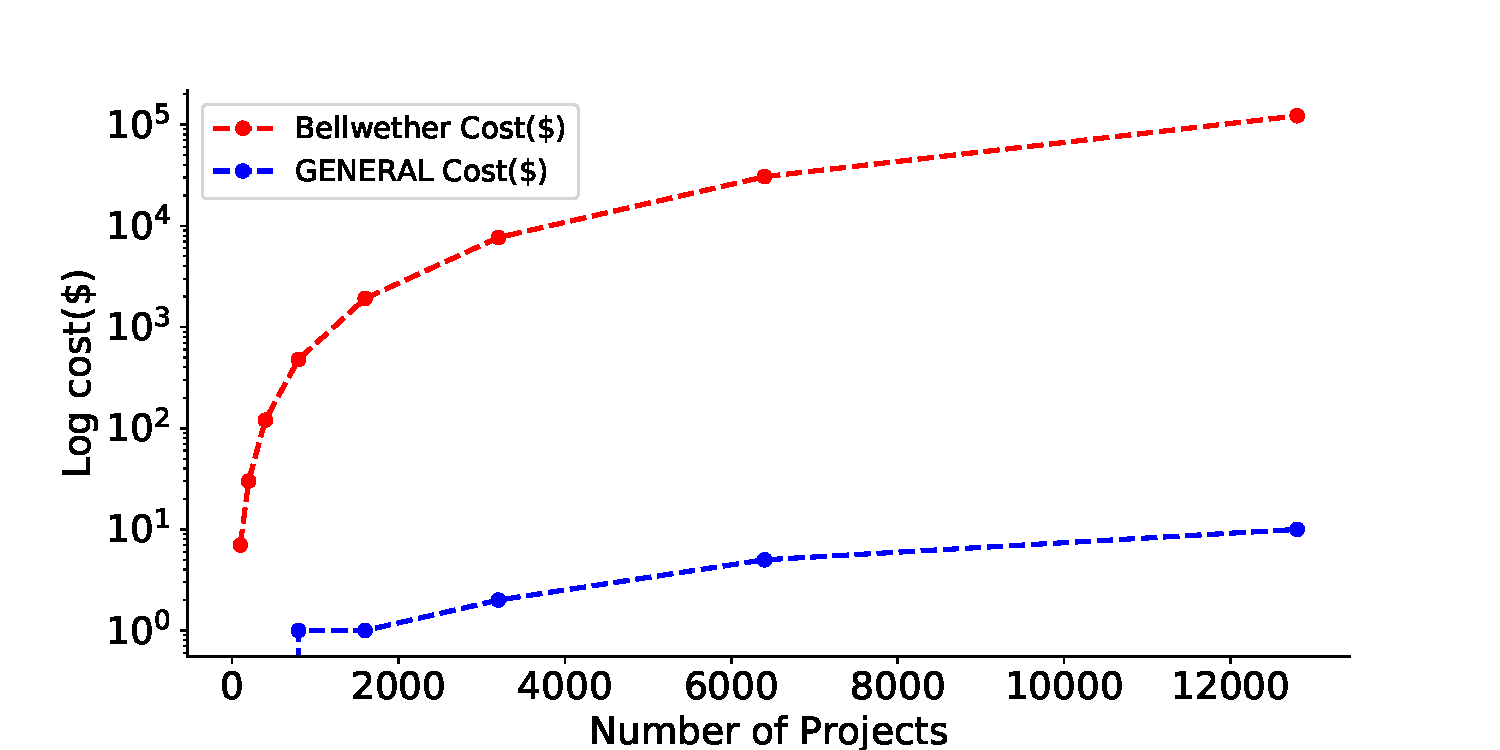
\includegraphics[width=\linewidth]{figs/cost.pdf}
%     \caption{Hypothetical cost comparison between GENERAL and default Bellwether.}
%     \label{fig:cost}
% \end{figure} 

% \noindent Overall, the  contributions of this paper are
% \bi

% \item \textbf{Hierarchical bellwethers for  transfer learner:} We
% offer a  novel hierarchical clustering    bellwether algorithm  called GENERAL  (described in section~\ref{GENERAL}) that
% finds bellwether in hierarchical clusters, then promotes those bellwether to upper levels
% The final  project that is promoted to the root of the hierarchy is returned as  ``the'' bellwether.

% \item \textbf{Showing inherent generality in SE:}
% In this study we discover a source data set for transfer learner from a large number of   projects, hence proving generality in the SE datasets (where some datasets can act as exemplars for the hundreds of other projects). To be more specific we can create a generalized defect prediction model that can act as a general model for rest of the projects in that SE community.

 




% \item \textbf{Knowledge   about software quality that are general
% to hundreds of software projects:}
%   As said above,    in  this sample of  697  projects,  we find that code  interface issues are the dominant factor on software defects. 



% In this section, we ask ``Why even bother to transfer knowledge   between projects?''. In several recent studies ~\cite{bettenburg2012think, menzies2012local, posnett2011ecological} with readily-available data from SE repositories, numerous authors report the locality effect in SE; i.e. general models outperformed by specialized models localized to particular parts of the data.
% For example.
% Menzies et al. explored local vs global learning in defect prediction and effort estimation~\cite{menzies2012local}  and found that
%  learning rules from specific local data was more
%  effective than learning rules from the global space.
 
 
% On the other hand, Herbold et al.~\cite{herbold2017global}  offered an opposite conclusion.
% In their   study regarding global vs local model for cross-project defect prediction,
% they saw that  local models offered little to no improvement over models learned
% from all the global data.
% One explanation for this discrepancy  is the size of number of projects that they explored.
% \respto{2-14}Menzies, Herbold et al. explored less than two dozen projects to their conclusions. Accordingly, here,  we explore nearly 700 projects to verify their findings. As shown below, the results of this paper agree  more with Herbold et al. than  Menzies et al. since we show that one global model (learned from a single bellwether projects) does just as well as anything else.
% \respto{2-14}Menzies, Herbold et al. explored less than two dozen projects which raises issues of external validity in their conclusions. Accordingly, here,  we explore nearly 700 projects. As shown below, the results of this paper agree  more with Herbold et al. than  Menzies et al. since we show that one global model (learned from a single bellwether projects) does just as well as anything else.

%\respto{2-24}{\color{blue} It turns out that developers are not the only one's confused about how various factors influence software projects. Much recent research calls into question  the ``established wisdoms'' of SE field. 


%Note that if the reader disputes any of the above, then we ask how would you challenge the items on this list? Where would you get the data, from enough projects, to   successfully refute the above? And where would you get that data? And how would you draw conclusions from that large set? Note that the answers to these questions requires learning from multiple projects. Hence, this paper.

%  Other researchers ~\cite{kocaguneli2012, kocaguneli2011find} doubted that a fixed value of k was appropriate for all data. That work recursively bi-clustered the source data, then pruned the cluster sub-trees with greatest ``variance'' (where the ``variance'' of a sub-tree is the variance of the conclusions in its leaves). This method combined row selection with row pruning (of nearby rows with large variance). Other similarity methods~\cite{Zhang16aa} combine domain knowledge with automatic processing: e.g. data is partitioned using engineering judgment before automatic tools cluster the data. To address variations of software metrics between different projects, the original metric values were discretized by rank transformation according to similar degree of context factors.

% \bi
% \item {\color{blue}Recall is the ratio between predicted actual target class examples vs all target class examples; i.e.  $ \frac{TP}{TP+FN} $, which means in an ideal scenario where we identify all the actual target class as target class without missing the recall will be one. 
% When recall is maximal, we are finding all  the target class.}
% \item  {\color{blue} Precision is the ratio between predicted actual target class examples vs all predicted target class examples; i.e. $ \frac{TP}{TP+FP} $. When precision is maximal, all the reports of defect modules are
% actually buggy (so the users waste no time looking at results that do not matter to them).}
% \item {\color{blue}popt(20) is a cost sensitive productivity based metric, which represents the percentage of total defect identified by reading 20\% of the code. This means more defects we can identify by reading only 20\% of the code is better for the developers to localize and fix the defects.}
% \item {\color{blue}ifa\_auc  is  XXX.}
% \ei

% In such   {\em multi-objective} problems, one model is better than another if it
%  satisfies a ``domination predicate''.
%  We use the Zitler indicator dominance
%  predictor~\cite{zit02} to select our bellwether (since this is known to select better models
%  for 5-goal optimization~\cite{Sayyad:2013,Sayyad:2013:SPL}).
% This predicate favors model
%   $y$ over $x$  model if $x$ ``losses'' most:
% \begin{equation}\label{eq:cdom}
% \begin{array}{rcl}
% \textit{worse}(x,y)& =& \textit{loss}(x,y) > \textit{loss}(y,x)\\
% \textit{loss}(x,y)& = &\sum_j^n -e^{\Delta(j,x,y,n)}/n\\
% \Delta(j,x,y,n) & = & w_j(o_{j,x}  - o_{j,y})/n
% \end{array}
% \end{equation}
% where  ``$n$'' is the number of objectives (for us, $n=5$) and $w_j\in \{-1,1\}$ depending on whether
% we seek to maximize goal $x_j$.  

% An alternative to the Zitler indicator is    `boolean domination ''
%  that says one thing is better than another it if it no worse on any criteria and better on at least one criteria. We prefer Equation~\ref{eq:cdom} to boolean domination since we
%  have a   5-goal optimization problem and it it is known that boolean domination often  fails for 3 or more goals~\cite{Wagner:2007,Sayyad:2013}. 
 

% The above equation is actually Pearson's correlation  where
% all variables have been standardized.  To be applied
% for discrete class learning (as done by KDP and this paper),
% Hall et al. employ the Fayyad Irani discretizer~\cite{FayIra93Multi} then apply the following
% entropy-based measure to infer $r$ (the degree of associations
% between  discrete sets $X$ and $Y$):

% \begin{equation}\label{eq:cfs}
% r_{\mathit{xy}}=2\times \left[ \frac{H(x) + H(y) - H(x,y)}{H(y)+H(x)} \right]
% \end{equation}
% where $H$ is the standard information gain measure used in 
% decision tree learning.
% \lstset{language=Python}
% \lstset{frame=lines} 
% \lstset{label={lst:code_direct}}
% \lstset{basicstyle=\footnotesize}
% \begin{center}\begin{minipage}{2.5in}\begin{lstlisting}
% def CFS(data):
%   features = []
%   score = -1
%   while True:
%     best = None
%     for feature in range(data.features):
%       features += [feature]
%       tmp = merit( data, features) # see above equation
%       if tmp > score:
%         score = tmp
%         bests = features
%       features.pop()
%     features += bests
%     if not improve(score): break
%   return features
% \end{lstlisting}
% \end{minipage}\end{center}
% \end{figure}


%  This algorithm works is  works in 6 stages.

%     (1) \textbf{Feature Extraction:} In this stage the whole dataset is used to extract features from each project. This is done using the FSS algorithm as shown in~\ref{subsec:FSS}. Here each project is sent to the FSS and the FSS returns most suitable features for building models, we do this for every project and that information as a vector (i.e. a vector or length equal to total number of features, where 0,1 represents a feature being absent,selected) that represents each project. By performing this we have a vector representation of each project in the dataset. GENERAL uses this information to create the hierarchical clusters to find the communities. We perceive this is a good representation of community, as in this work we try to find community which has similar information distribution according to the attributes. Thus 2 projects with similar features selected have much higher chance of building similar models.
    
%     (2) \textbf{Cluster Creation:} After the feature extraction has been done, the data is sent to a modified BIRCH algorithm. The algorithm requires a branching factor (i.e. Maximum number of CF sub-clusters in each node) and threshold value (i.e. when to form a new cluster based on radius). For this experiment we have set the branching factor as 20 and threshold value as 0.5. Using this version of BIRCH algorithm we build the hierarchical cluster, while storing all necessary details about the cluster like parent-child node, data points, level information, etc. This stage returns a Clustering Feature Tree (CF Tree) with all this information, which is passed to the next phase of experiment. 
    
%     (3) \textbf{Bellwether selection phase 1:} The CF Tree from the last phase is passed to the hierarchical bellwether. In this phase we use \textit{bellwether method} to identify bellwether at the leaf level. Using the CF Tree, we identify the clusters at the leaf level where each cluster represents the smallest community produced by the BIRCH algorithm in the last phase. Here we use the default ``Bellwether'' to perform a $ N*(N-1) $ comparison at each cluster. Here we select each project in the cluster one by one as a source dataset for transfer learning apply SMOTE as mentioned in sec~\ref{subsec:SMOTE} to handle any data imbalance and then use the FSS algorithm to get rid of any unnecessary attributes as mentioned in sec~\ref{subsec:FSS}. This informative and balanced dataset is used to build a LR model as mentioned in sec~\ref{subsec:LR} and we measure the performance of all other projects in the community (cluster). The performance measures that are used are mentioned in sec~\ref{sec:Measures}. To find the bellwether in each community we use cdom function to find the best source dataset among each cluster considering all performance measures. This phase returns a bellwether for each cluster at the leaf level of the CF Tree.
    
%     (4) \textbf{Bellwether promotion:} In this phase of the algorithm is an iterative process, here we receive the selected bellwethers from the child clusters of each cluster in the level. This is called the bellwether promotion. Here each parent cluster instead of being represented by all projects within them, they are represented by only the bellwethers in them.  
    
%     (5) \textbf{Bellwether selection phase 2:} In this phase instead of finding a bellwether for each cluster at the level by performing a $ N*(N-1) $ comparison, we select the projects which represented as bellwether at the child nodes and then try to find a bellwether among them. So at each cluster at the level we perform a $ M*(M-1) $ comparison at each cluster where M is the selected bellwether from child clusters. This creates an order of magnitude faster \textbf{bellwether method}. This is again an iterative process, and the end of all the iterations, we will have a bellwether at each cluster at every level. 
    
%     (6) \textbf{Bellwether Prediction:} This is the transfer learning phase, when a new project is evaluated, we will use the FSS algorithm to get its features, then use the feature vectors to identify which cluster it belongs and use that cluster's bellwether as the transfer learning model.

% \begin{figure}[!t]
%     \centering
%     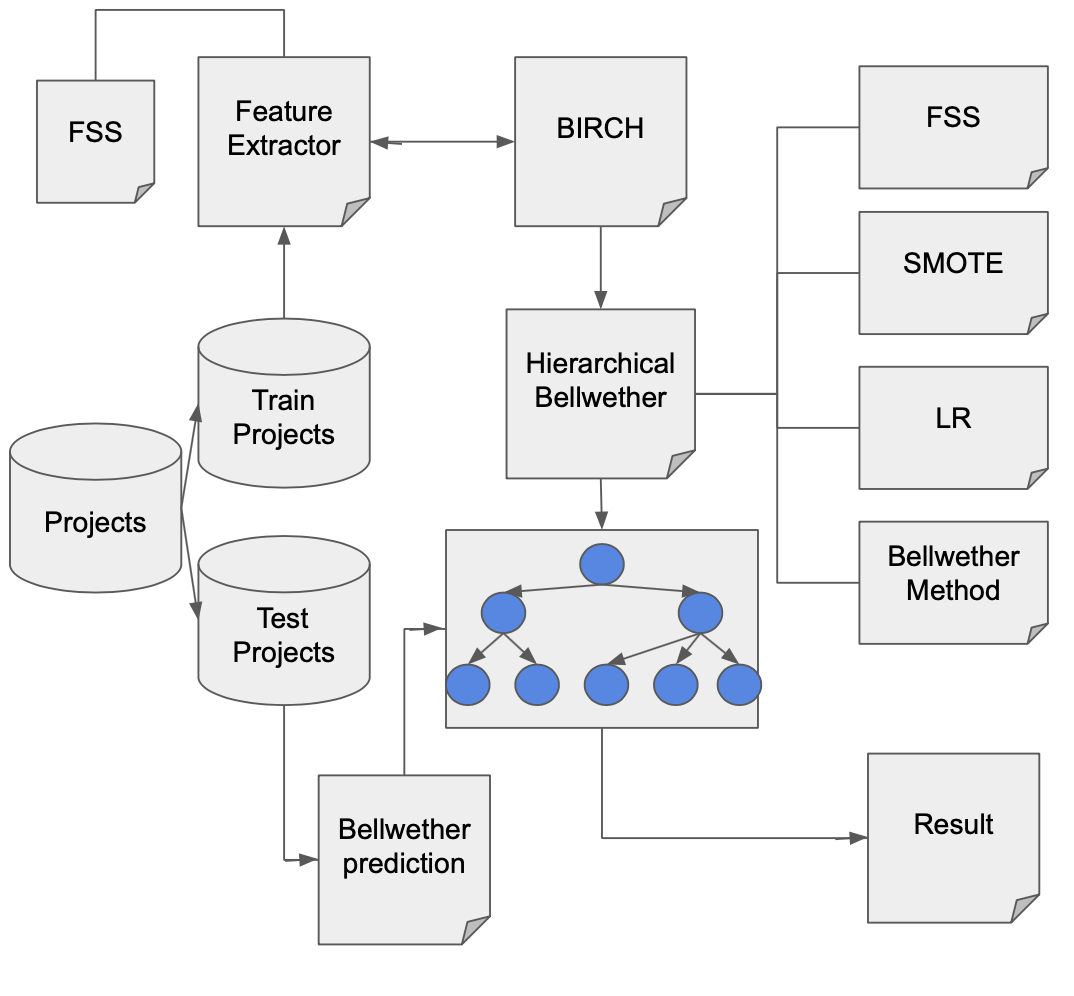
\includegraphics[width=\linewidth]{figs/BUBBLE.png}
%     \caption{GENERAL algorithm.}
%     \label{fig:GENERAL}
% \end{figure}

% In this study we try to establish the presence of generality in SE datasets. We do this by analyzing the presence of bellwether incrementally by adding more and more projects and how the bellwether's predictive power changes. In this case to show the presence of generality in SE datasets the predictive power of the bellwether should look like the \textcolor{ao(english)}{GREEN} in figure~\ref{fig:predictive_power}, that is the predictive power of bellwether should increase or remains same, if our results look like the \textcolor{red}{RED} curve, that will show absence of generality in SE datasets.

% In order to achieve this, we try to explore the \textit{bellwether effect} as mentioned in ~\ref{sec:related}. We know the default \textit{bellwether method} is very expensive ($ O(N^2) $). Thus in this paper we proposes an alternative transfer learning method (GENERAL), that explores \textit{bellwether effect} by exploring an order of magnitude faster \textit{bellwether method}. Our approach has three key components:

% \bi

%     \item A feature extractor to find a representation of each project, which will be used for clustering the projects. 
    
%     \item A hierarchical clustering model to use the features extracted from previous step to build the hierarchical cluster.
    
%     \item A transfer learning model to identify bellwether in the hierarchical cluster.

% \ei

% GENERAL employs a few different algorithms to complete and compose it's 4 different components - 

% \subsubsection{\textbf{Feature Subset Selection (FSS):}}
% \label{subsec:FSS}
% To extract features from each dataset, we use a feature selector algorithm called Feature Subset Selection(FSS)~\cite{hall1999correlation,hall1997feature}. Which is a process of identifying and removing as much irrelevant and redundant information as possible. This is achieved using a correlation based feature evolution strategy to evaluate importance of an attribute and a best first search strategy with backtracking that moves through the search space by making local changes to the current feature subset. Here if the path being explored begins to look less promising, the best first search can back-track to a more promising previous subset and continue the search from there. Given enough time, a best first search will explore the entire search space, so it uses a stopping criterion (i.e. no improvement for five consecutive attributes).

% {\small 
% \begin{figure}[]
%     \small 
%     \inputminted[numbersep=2pt, linenos=true, fontsize=\small]{python}{pseudocode/cfs.py}
%     \vspace{-0.2cm}
%     \caption{Pseudo-code of Feature Subset Selection}
%     \label{fig:GAP_pseudocode} 
%     \vspace{-0.3cm}
% \end{figure}
% } 


% \subsection{Performance Measures}
% \label{sec:Measures}

% In this section, we introduce the following 5 evaluation measures used in this study to evaluate the performance of machine learning models. Suppose we have a dataset with M changes and N defects. After inspecting 20\% LOC, we inspected $m$ changes and found $n$ defects. Also, when we find the first defective change, we have inspected k changes. Using
% this data, we can define 5 evaluation measures  as follows:

% (1) \textbf{Recall:} This is the proportion of inspected defective changes among all the actual defective changes; i.e. $n/N$.
% Recall is used in  many previous studies~\cite{kamei2012large,yang2016effort,yang2017tlel,xia2016collective,yang2015deep}.  

% (2) \textbf{Precision:} This is the proportion of inspected defective changes among all the inspected changes; i.e. $n/m$. A low Precision indicates that developers would encounter more false alarms, which may have negative impact on developers' confidence on the prediction model.  

% (3) \textbf{pf:} This is the proportion of all suggested defective changes which are not actual defective changes among all the suggested defective changes. A high {\em pf} suggests developers will encounter more false alarms which may have negative impact on developers' confidence in the prediction model.

% (4) \textbf{popt20:} This is the proportion number of suggested defective changes among all suggested defective changes, when when 20\% LOC modified by all changes are inspected. 
% A high {\em popt20} values mean that developers can find most bugs in a small percent of the code.
% To compute Popt20, we divided the test set into the modules predicted to be faulty (set1)
% and predicted to be bug-free (set2). Each set was then sorted in ascending order by lines 
% of code.  We then ran down set1, then set2, till 20\% of the total lines of code
% were reached-- at which point {\em popt20} is the percent of buggy modules seen up to that point.

% (5) \textbf{ifa\_auc:} Number of  initial false alarms encountered before we find the first defect. Inspired by previous studies on fault localization~\cite{parnin2011automated, kochhar2016practitioners, xia2016automated}, we caution that if the top-k changes recommended by the model are all false alarms, developers would be frustrated and are not likely to continue inspecting the other changes. Parnin and Orso ~\cite{parnin2011automated} found that developers would stop inspecting suspicious statements, and turn back to traditional debugging, if they could not get promising results within the first few statements they inspect. Using the nomenclature reported about {\em ifa$=k$}.  In this study we use a modified version of {\em ifa} called ifa\_auc, which calculates {\em ifa} based on efforts spent on inspecting the code. We use gradually increment the efforts spent by increasing the total LOC inspected and calculate ifa on each iteration to get the area under the curve (auc), here the x-axis is the percentage of effort spent on inspection and y-axis is {\em ifa}.

% In the literature, we saw most of the previous studies have shown bellwether effect with very small datasets. In order to use bellwether to prove presence of generality in SE domain datasets, we first have to showcase the bellwether method suggested by Krishna et al. in their experiment works for large datasets. We use our defect prediction dataset with 697 projects for this purpose. 

% We divide the dataset in train\_1 and test\_1 set and then performed a $ N*(N-1) $ comparison on all the projects in train\_1 set to find a bellwether, and then dividing each project in test\_1 set into train\_2 and test\_2 using a train\_test split. We use the train\_2 to train a LR model and test on test\_2 which is represented as \textit{self} in the figures. Similarly we use the bellwether project from train\_1 to train a LR model and test it on test\_2 which is represented as \textit{bellwether0}. We use statistical tests mentioned in section~\ref{stats} to compare the performance of \textit{self} vs \textit{bellwether0} for all the performance measures mentioned in section~\ref{sec:Measures}, which is shown 

% \begin{figure}[!b]
%     \centering
%     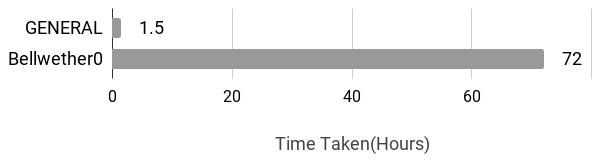
\includegraphics[width=\linewidth]{figs/Time.png}
%     \caption{Mean run-time for for one run of standard bellwether and GENERAL (With SMOTE and CFS).}
%     \label{fig:time}
% \end{figure}

% \fig{compare} shows the mean number of comparisons required for finding a bellwether using conventional bellwether versus GENERAL for different community size of 45,90, 180, 360 and 627 projects. We can see from the \fig{compare} for increasing community size the number of comparisons required increases rapidly for conventional bellwether, while with GENERAL the number of comparisons required are relatively small. This shows the new bellwether method (aka GENERAL) is scalable with increasing community size. 

% similarly \fig{compare_time} shows the mean run times for one run of GENERAL versus traditional bellwether for different community size of 45,90, 180, 360 and 627 projects. It is evident from the figure with growing community size the new bellwether method takes lesser amount of time ($\approx 4$ times faster in community size of 50 while $\approx 30$ times faster in a community size of 627 projects ).

% %%%%%%%%%%%%%%%%%%%%%%%%%%%%%%%%%%%%%%%%%%%%%%%%%%%%%%%%%%%
% %%%%%%%%%%%%%%%%%%%%%%%Latex Table%%%%%%%%%%%%%%%%%%%%%%%%%
% \begin{figure}[!b]
% {\scriptsize
% {\scriptsize \begin{tabular}{p{.1cm}lp{1.5cm}rrc}
% \arrayrulecolor{darkgray}
% \rowcolor[gray]{.9}  & rank & treatment & mean & sd & \\
%  \multirow{5}{*}{\rotatebox[origin=c]{90}{Recall}} 
%   &   1 &      GENERAL\_level2 &    38 &  32 & \quart{22}{38}{32}{16} \\
%   &   1 &      bellwether0 &    39 &  31 & \quart{23}{39}{31}{15} \\
%   &   1 &  ZeroR &    40 &  49 & \quart{16}{40}{49}{25} \\
%   &   2 &      GENERAL\_level1 &    48 &  33 & \quart{31}{48}{33}{16} \\
%   &   3 &      self &    55 &  27 & \quart{41}{55}{27}{12} \\
%   &   3 &      GENERAL\_level0 &    56 &  31 & \quart{42}{56}{31}{16} \\
%   &   4 &      global &    78 &  40 & \quart{57}{78}{40}{20} \\ \hline
% \multirow{5}{*}{\rotatebox[origin=c]{90}{Pf}} 
%   &  1 &      GENERAL\_level2 &    28 &  28 & \quart{14}{28}{28}{13} \\
%   &  1 &      bellwether0 &    28 &  25 & \quart{15}{28}{25}{11} \\
%   &  1 &      self &    30 &  20 & \quart{20}{30}{20}{10} \\
%   &  1 &      GENERAL\_level1 &    35 &  28 & \quart{21}{35}{28}{14} \\
%   &  1 &      ZeroR &    39 &  49 & \quart{15}{39}{49}{25} \\
%   &  2 &      GENERAL\_level0 &    47 &  31 & \quart{31}{47}{31}{15} \\
%   &  3 &      global &    79 &  39 & \quart{59}{79}{39}{19} \\\hline
% \multirow{5}{*}{\rotatebox[origin=c]{90}{Precision}} &   1 &      ZeroR &    21 &  30 & \quart{6}{21}{30}{15} \\
%     &  2 &      global &    35 &  28 & \quart{21}{35}{28}{14} \\
%     &   2 &      GENERAL\_level2 &    39 &  34 & \quart{22}{39}{34}{17} \\
%     &   2 &      bellwether0 &    40 &  33 & \quart{23}{40}{33}{16} \\
%     &   2 &      GENERAL\_level1 &    42 &  31 & \quart{26}{42}{31}{15} \\
%     &   2 &      GENERAL\_level0 &    44 &  30 & \quart{28}{44}{30}{15} \\
%     &   2 &      self &    50 &  30 & \quart{35}{50}{30}{15} \\\hline
% \multirow{5}{*}{\rotatebox[origin=c]{90}{Popt20}} &   1 &      ZeroR &    13 &  16 & \quart{5}{13}{16}{8} \\
%   & 2 &      GENERAL\_level2 &    26 &  22 & \quart{15}{26}{22}{11} \\
%   &  2 &      global &    26 &  13 & \quart{19}{26}{13}{6} \\
%   &  2 &      bellwether0 &    28 &  21 & \quart{17}{28}{21}{9} \\
%   &  2 &      GENERAL\_level0 &    28 &  15 & \quart{22}{28}{15}{8} \\
%   &  2 &      GENERAL\_level1 &    28 &  19 & \quart{19}{28}{19}{9} \\
%   &  3 &      self &    35 &  19 & \quart{26}{35}{19}{10} \\\hline
% \multirow{5}{*}{\rotatebox[origin=c]{90}{ifa\_auc}} &   1 &      ZeroR &    7 &  11 & \quart{1.12}{6.77}{11.29}{5.65} \\
%   &  2 &      global &    19 &  16 & \quart{11.35}{19.38}{16.06}{8.03} \\
%   &  3 &      GENERAL\_level2 &    22 &  14 & \quart{14.48}{21.59}{14.21}{7.10} \\
%   &  3 &      bellwether0 &    23 &  14 & \quart{15.48}{22.56}{14.15}{7.07} \\
%   &  3 &      self &    23 &  12 & \quart{17.09}{22.93}{11.68}{5.84} \\
%   &  3 &      GENERAL\_level1 &    23 &  14 & \quart{16.10}{22.98}{13.74}{6.87} \\
%   &  3 &      GENERAL\_level0 &    25 &  13 & \quart{17.87}{24.51}{13.27}{6.63} \\
% \end{tabular}}
% }
% \caption{Statistical Results comparison. The ``rank`` column at left comes from
% the statistical analysis methods of \S\ref{eval}. Note that for {\em pf}, and {\em ifa} rank=1 is the best rank while for all other performance measures, ranks $\in{3,4}$ are best. 
% }\label{fig:Statistical}
% \end{figure}

% {\small 
% \begin{figure*}[!t]
%     \centering
%     \begin{tikzpicture}[nodes={draw, circle,fill=darkgray!60}, ->,sibling distance=.7cm,minimum size=.1cm,scale=.5]
 
%     \node{627}
%         child { node {57}
%             child {node {9}} 
%             child {node {9}} 
%             child {node {7}} 
%             child {node {17}}
%             child {node {13}}}
%         child [missing]
%         child [missing]
%         child [missing]
%         child [missing]
%         child [missing]
%         child [missing]
%         child [missing]
%         child { node {127} 
%             child {node {3}} 
%             child {node {9}} 
%             child {node {19}} 
%             child {node {15}}
%             child {node {4}}
%             child {node {17}} 
%             child {node {15}} 
%             child {node {19}} 
%             child {node {11}}
%             child {node {15}}}
%         child [missing]
%         child [missing]
%         child [missing]
%         child [missing]
%         child [missing]
%         child [missing]
%         child [missing]
%         child [missing]
%         child [missing]
%         child [missing]
%         child [missing]
%         child [missing]
%         child { node {183} 
%             child {node {8}} 
%             child {node {3}} 
%             child {node {12}} 
%             child {node {16}}
%             child {node {20}}
%             child {node {18}} 
%             child {node {12}} 
%             child {node {4}} 
%             child {node {12}}
%             child {node {16}}
%             child {node {5}}
%             child {node {17}} 
%             child {node {9}} 
%             child {node {9}} 
%             child {node {10}}
%             child {node {14}}}
%         child [missing]
%         child [missing]
%         child [missing]
%         child [missing]
%         child [missing]
%         child [missing]
%         child [missing]
%         child [missing]
%         child [missing]
%         child [missing]
%         child [missing]
%         child [missing]
%         child [missing]
%         child [missing]
%         child [missing]
%         child [missing]
%         child [missing]
%         child { node {260} 
%             child {node {17}} 
%             child {node {17}} 
%             child {node {20}} 
%             child {node {14}}
%             child {node {9}}
%             child {node {13}} 
%             child {node {18}} 
%             child {node {10}} 
%             child {node {18}}
%             child {node {10}}
%             child {node {6}} 
%             child {node {15}} 
%             child {node {14}} 
%             child {node {9}}
%             child {node {10}}
%             child {node {8}} 
%             child {node {7}} 
%             child {node {13}} 
%             child {node {15}}}
%             ;
% \end{tikzpicture}
%     \caption{Example of Hierarchical Clustering for 627 projects}
%     \label{fig:example tree}
% \end{figure*}
% }

% As to {\em ZeroR}, we cannot recommend that approach.
% While {\em ZeroR} 
% makes few mistakes (low {\em ifa}s and low {\em pf}s), it scores badly
% on   other measures (very low {\em recall}s  and {\em popt(20)}.



% In this section, we return to 
% In RQ4, we try to answer the question if learning from too many projects detrimental effect, this question has two parts, one on predictive power, the other on making general conclusion and conclusion instability. Figure~\ref{fig:Statistical} shows the results of statistical significance and effect size tests to rank them in order for all the different methods(treatments) used in this experiment. In this figure for a performance measure two methods showing same rank means there performance is not statistically significantly different, while a different ranks mean they are different, while a smaller rank is better if the performance goal is negative (i.e. Pf), and higher rank is better in case of positive goal (i.e. Recall).

% To answer the first part of the question, if learning from too many projects have detrimental effect on predictive power of models, we compare the results of default ``bellwether method'' (a.k.a bellwether0) proposed by Krishna et al. and GENERAL(a.k.a GENERAL\_level0) method. The results of scott-knott test shows that for positive goals such as Recall the GENERAL\_level0 is significantly doing better than Bellwether0 and it is doing as good as or better for precision ans recall. While for negative goals such as ifa\_auc GENERAL\_level0 is doing as good as bellwether0. Although in case of Pf they score different ranks with GENERAL showing higher Pf then bellwether0, it is not by much. Similarly while comparing GENERAL\_level0 with global (which is learning from all the projects) shows although it achieves higher Recall, but it has very high Pf, low precision. Which answers the first part of the question that learning from too many projects do have detrimental effect on predictive power of models. 


% Now to answer the second part of the question, that is if learning from too many projects creates conclusion instability, we will look at figure~\ref{fig:FSS_compare}. Figure~\ref{fig:FSS_compare} show the distribution of attributes selected while building a ML model for defect prediction using local models(a.k.a self), the \textcolor{red}{{\bf red bars}} shows the attributes selected by the ``Bellwether Project''. Conclusion instability causes vastly different and often contradicting conclusions to be derived from a data source. This sort of instability is very prevalent in several domains of software engineering. We can see from figure~\ref{fig:FSS_compare}, when learning from local data, each model selected different sets of attributes and resulted in selecting almost all different attributes. That means there is no general conclusion can be drawn for defect prediction models by saying which attributes are important, this results in conclusion instability and that effects the trusts on those models, the insights that can be drawn from them. Which farther affects training and tool development as mentioned in sec~\ref{sec:Motivation}. From these results we can see learning from too many data can cause conclusion instability and thus affecting generality in SE domain. In Summary, we can say 



% \begin{figure*}[h]
%     \centering
%     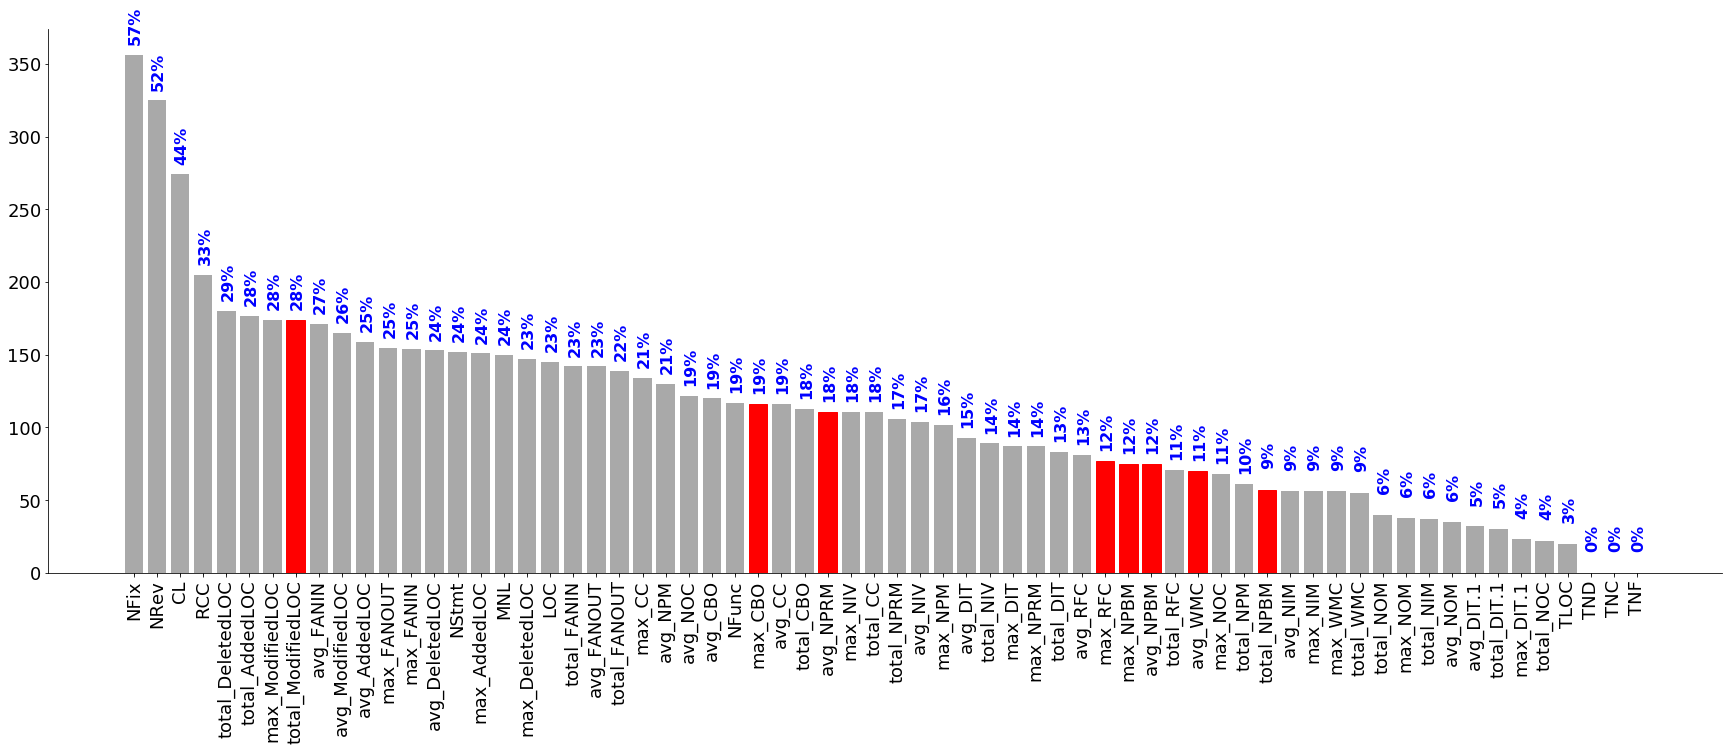
\includegraphics[width=\linewidth]{figs/FSS_compare.png}
%     \caption{Distribution of features selected using self model and ``Bellwether'' model.}
%     \label{fig:FSS_compare}
% \end{figure*}


% \begin{figure*}
%         \centering
%         \begin{subfigure}[b]{0.475\textwidth}
%             \centering
%             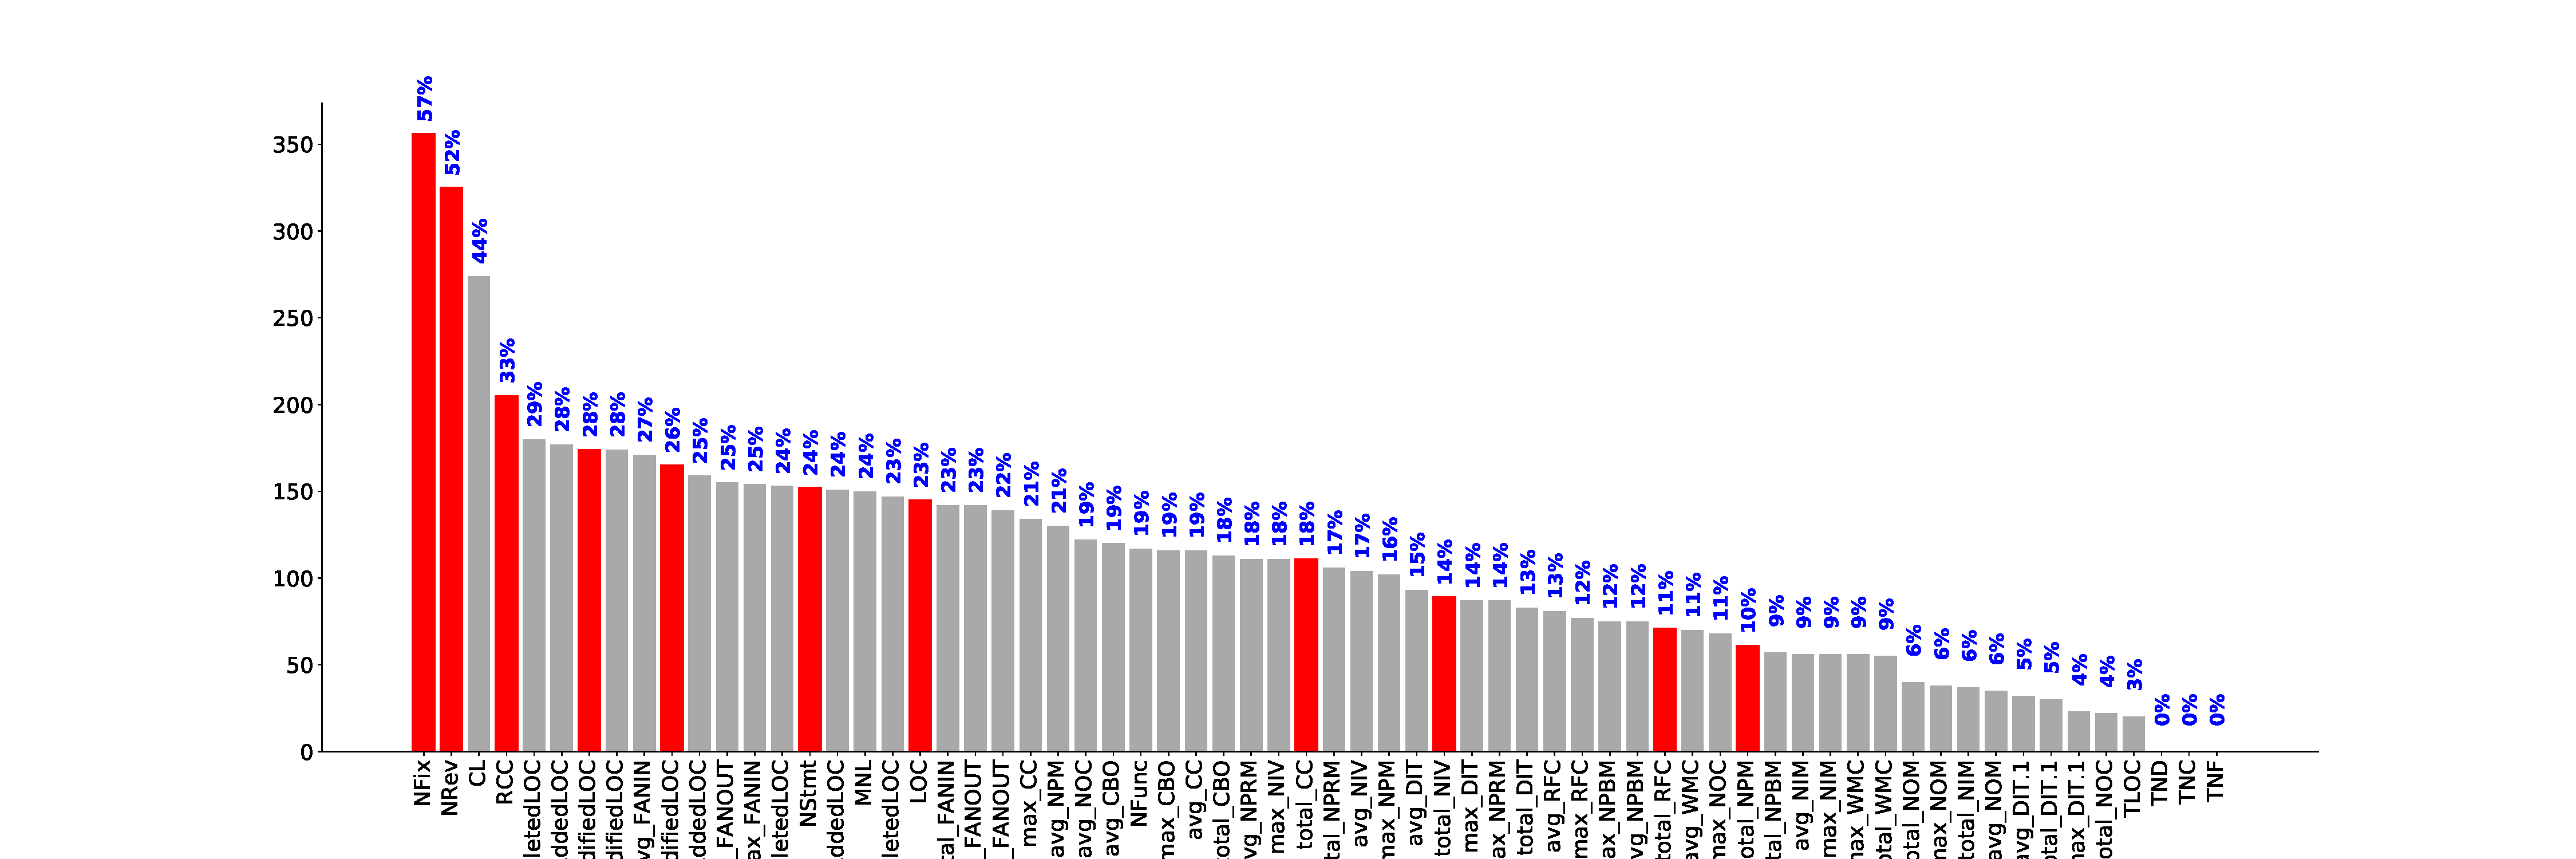
\includegraphics[width=\textwidth]{figs/fss_all0.pdf}
%             \caption[Network2]%
%             {{\small Network 1}}    
%             \label{fig:mean and std of net14}
%         \end{subfigure}
%         \hfill
%         \begin{subfigure}[b]{0.475\textwidth}  
%             \centering 
%             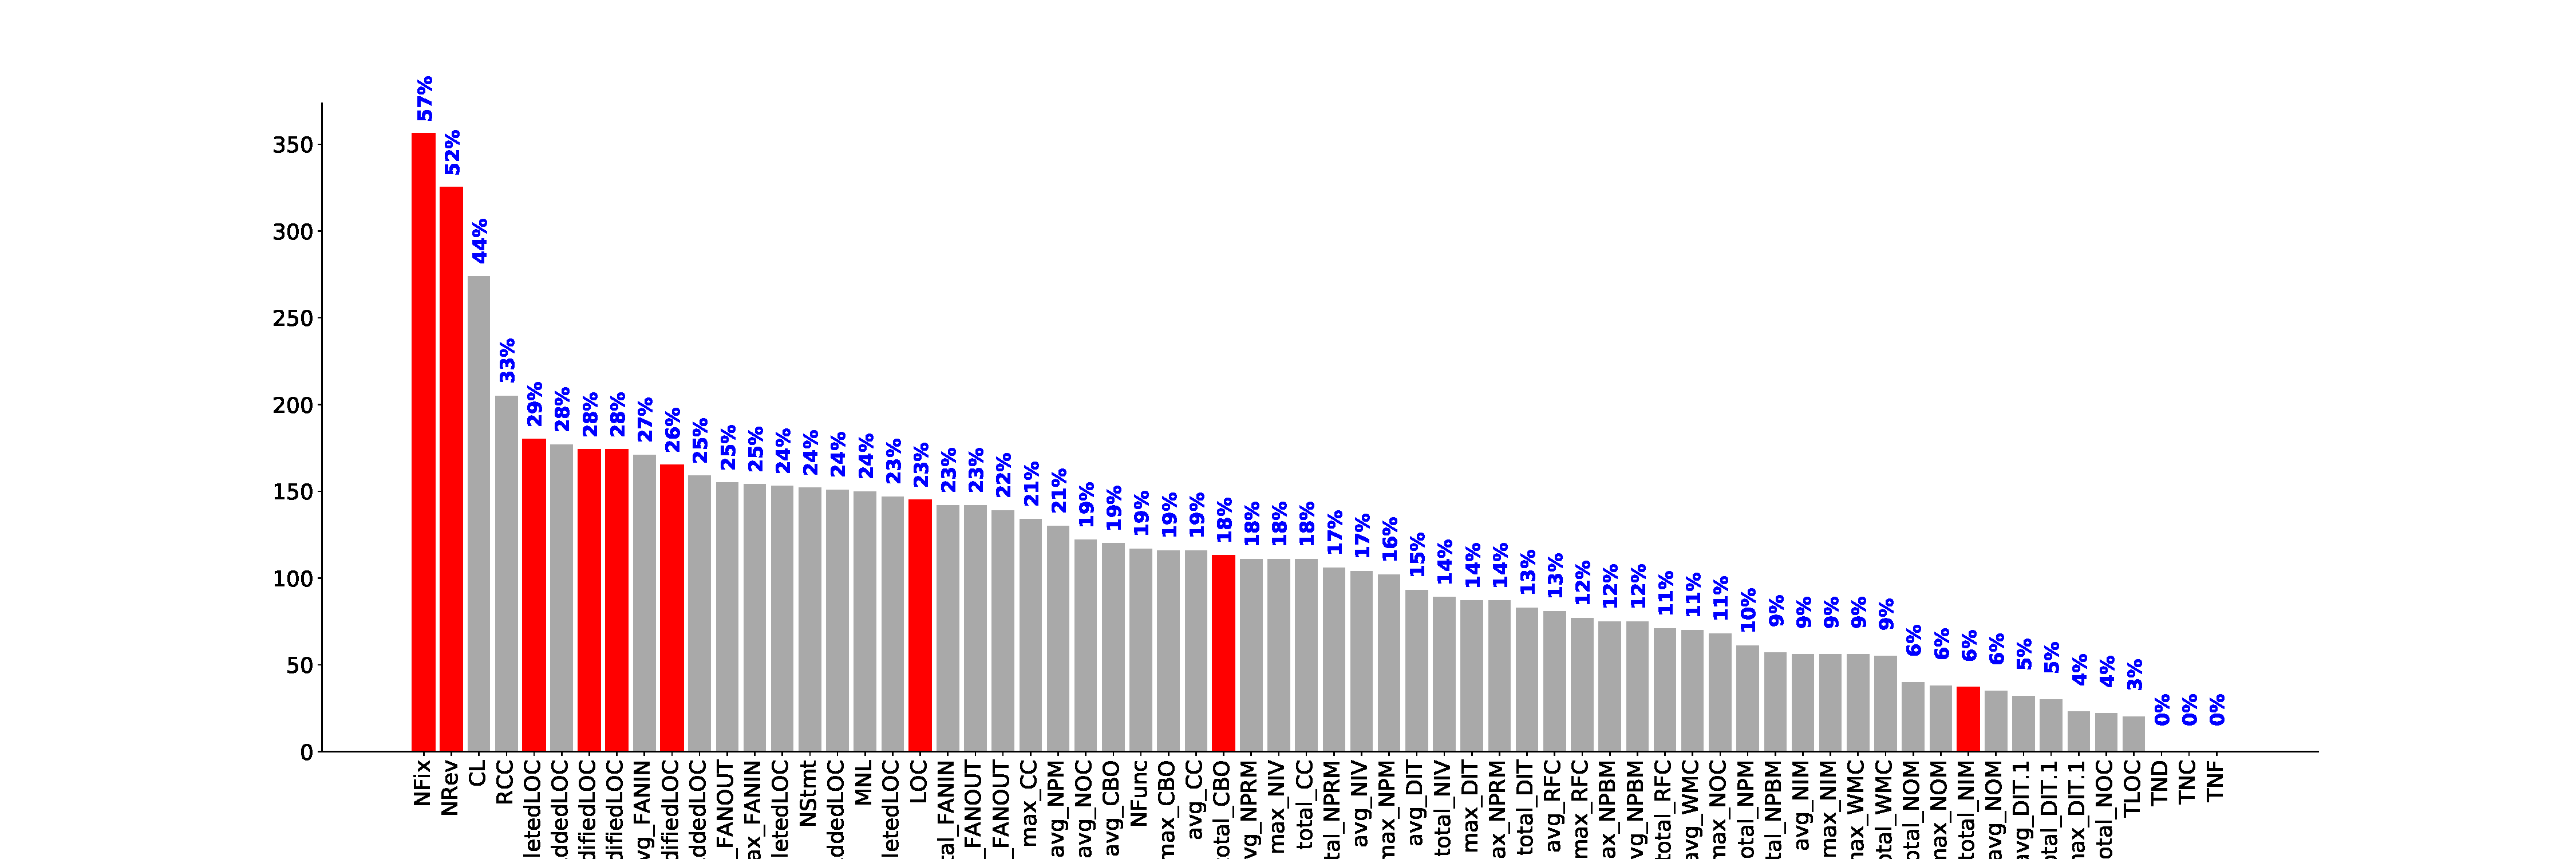
\includegraphics[width=\textwidth]{figs/fss_all1.pdf}
%             \caption[]%
%             {{\small Network 2}}    
%             \label{fig:mean and std of net24}
%         \end{subfigure}
%         \vskip\baselineskip
%         \begin{subfigure}[b]{0.475\textwidth}   
%             \centering 
%             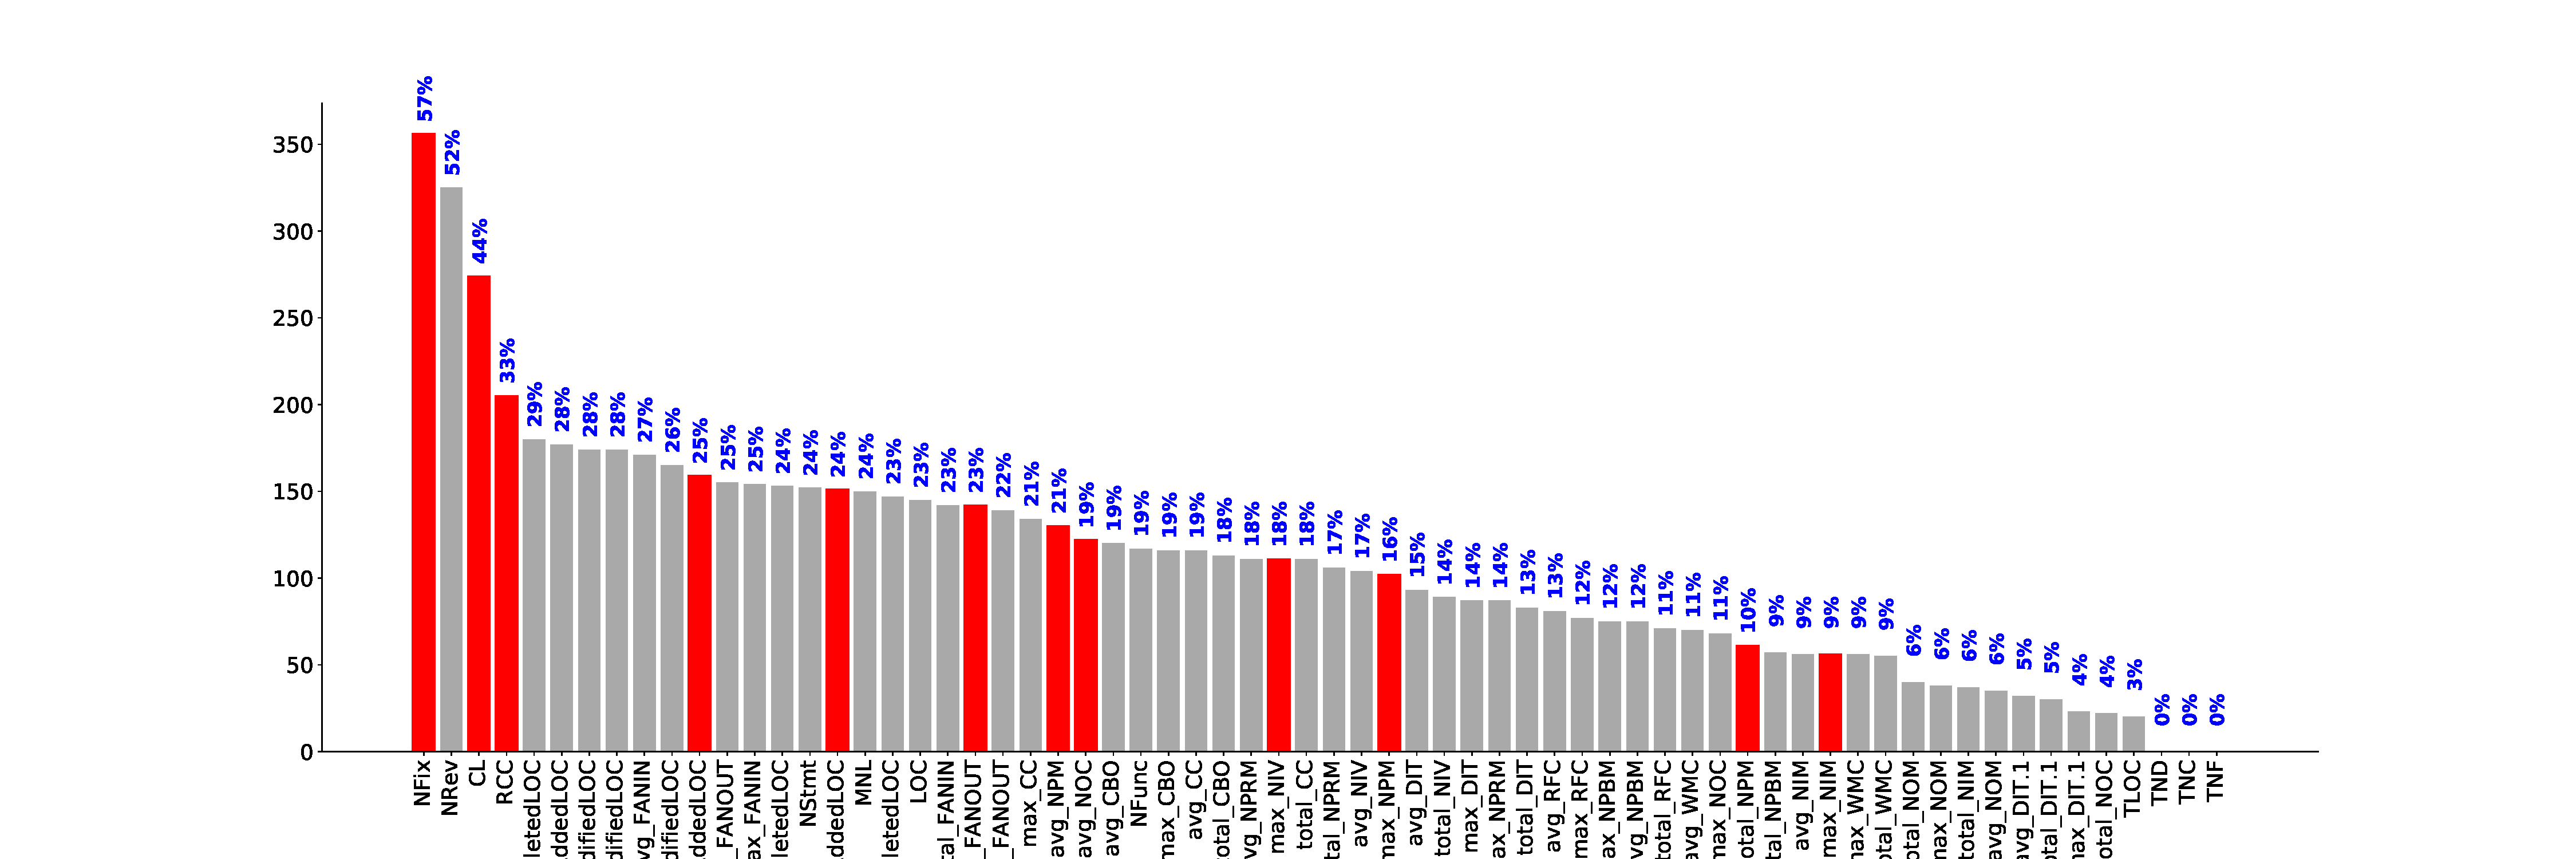
\includegraphics[width=\textwidth]{figs/fss_all2.pdf}
%             \caption[]%
%             {{\small Network 3}}    
%             \label{fig:mean and std of net34}
%         \end{subfigure}
%         \quad
%         \begin{subfigure}[b]{0.475\textwidth}   
%             \centering 
%             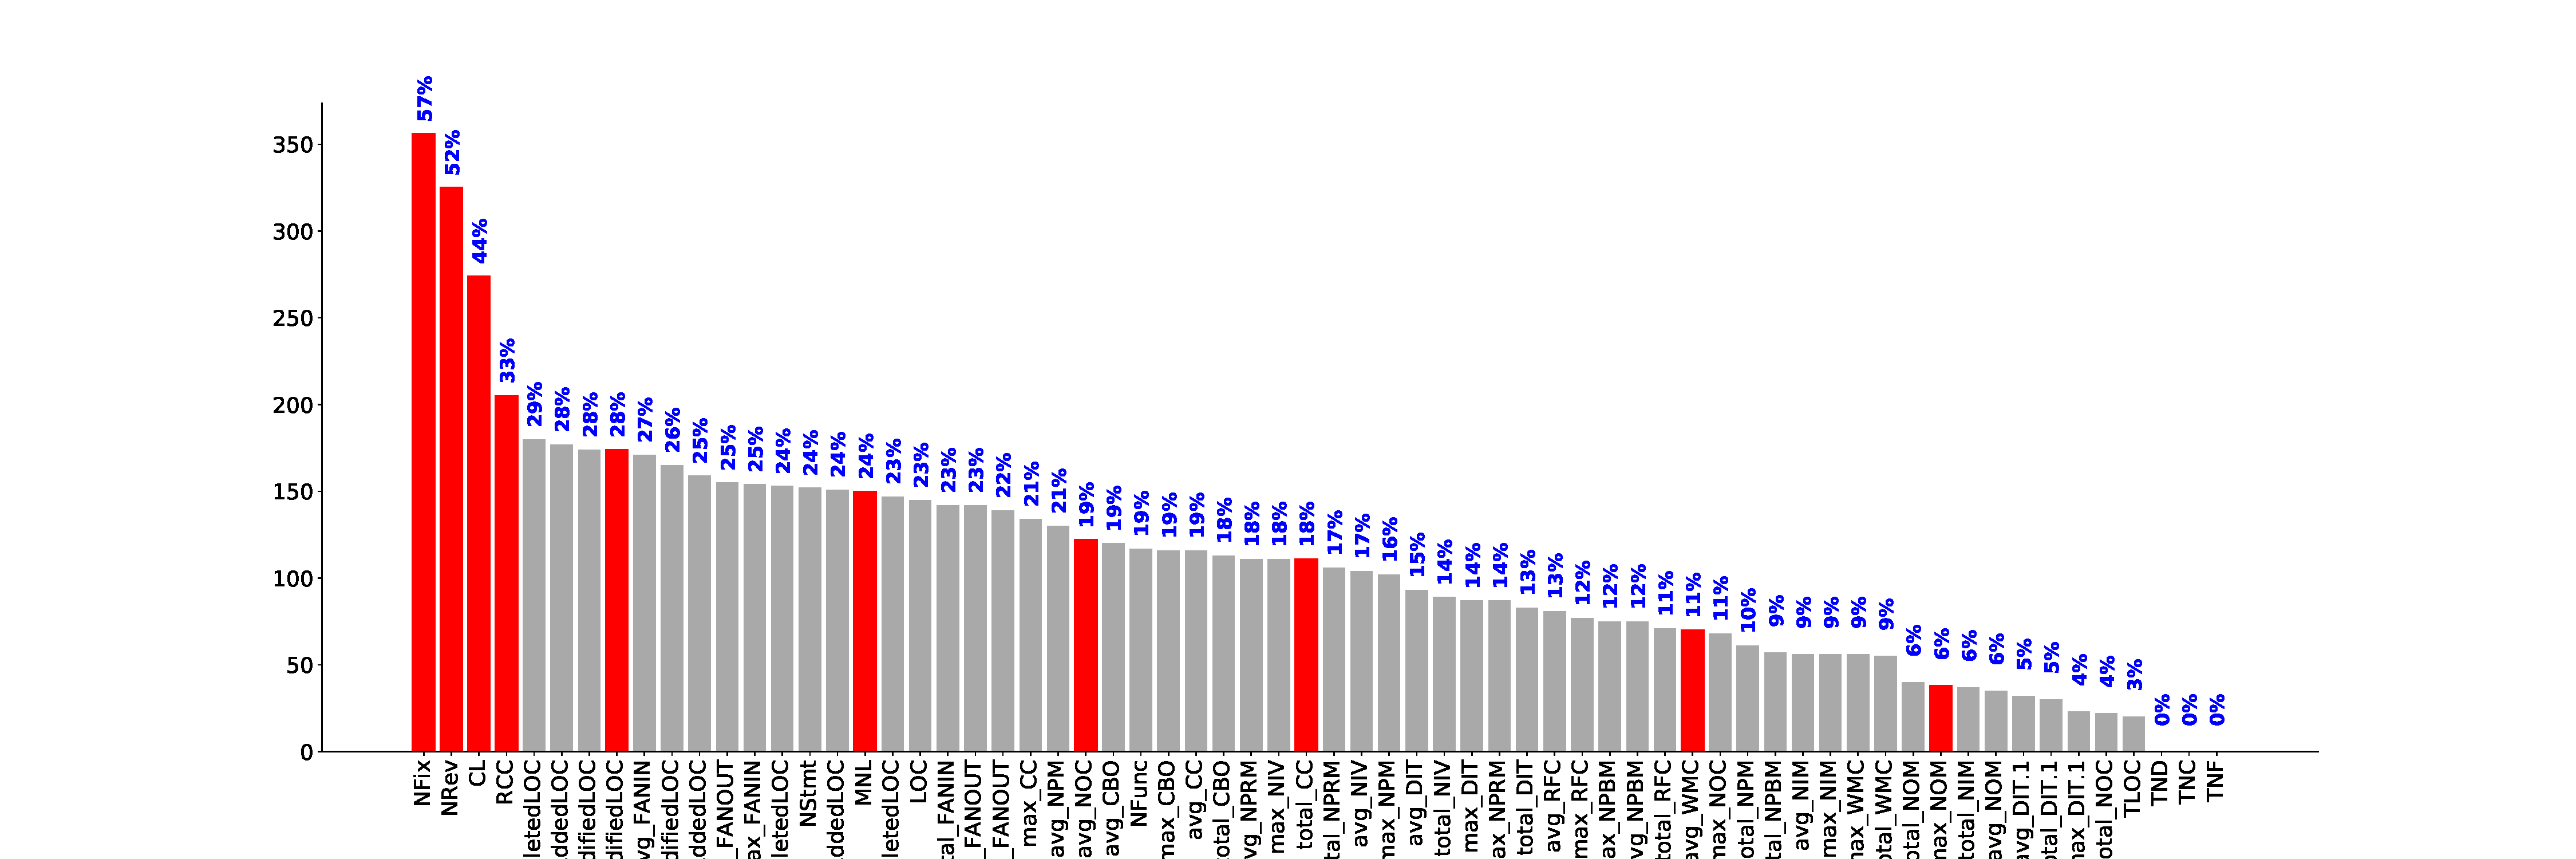
\includegraphics[width=\textwidth]{figs/fss_all3.pdf}
%             \caption[]%
%             {{\small Network 4}}    
%             \label{fig:mean and std of net44}
%         \end{subfigure}
%         \caption[ The average and standard deviation of critical parameters ]
%         {\small The average and standard deviation of critical parameters: Region R4} 
%         \label{fig:mean and std of nets}
%     \end{figure*}

% \begin{figure*}[]
%     \centering
%     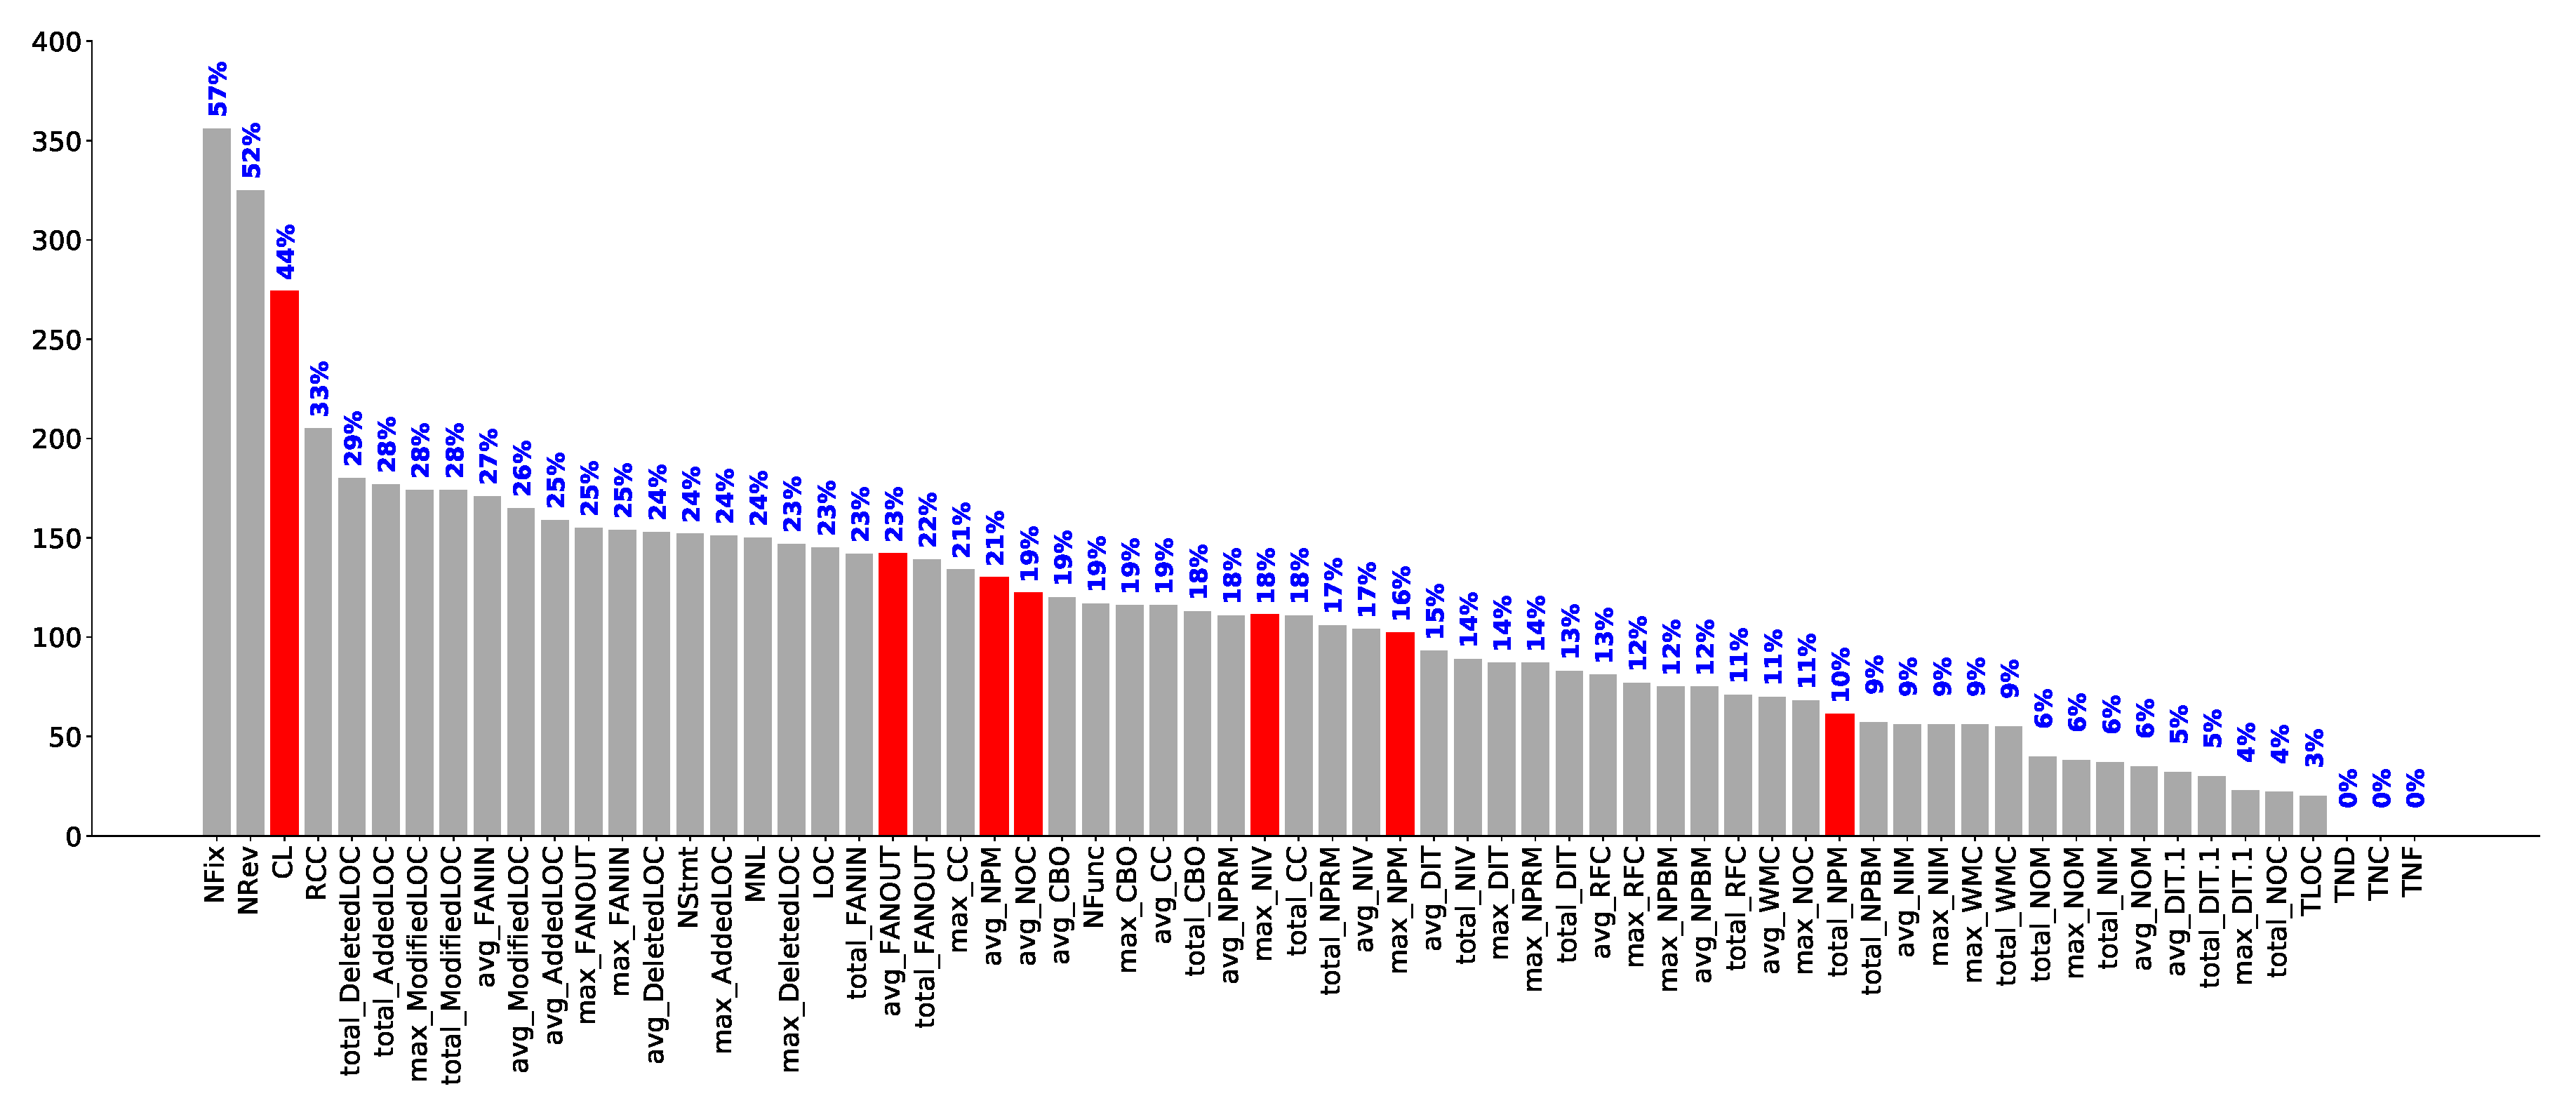
\includegraphics[width=\linewidth]{figs/fss_1.pdf}
%     \caption{Distribution of features selected using self model and ``Bellwether'' model.}
%     \label{fig:FSS_level0}
% \end{figure*}

% \subsection*{RQ6: What exactly did we learn from all those projects?}
% \label{sec:rq6}

% Having demonstrated that we can quickly find bellwethers
% from hundreds of software projects, it is appropriate to ask
% what model was learned from all that data. This is an important question for this research since if  we cannot show the lessons
% learned from our 627 projects, then all the above is wasted effort.

% Table~\ref{tbl:coefs}  shows the weights learned by logistic
% regression after feature selection using the bellwether project
% selected by {\em GENERAL\_level0}. Note that:
% \bi
% \item
% The number of features that appear in Table~\ref{tbl:coefs}  is much smaller than the list of features shown in Table~\ref{tbl:metric}.
% That is, our bellwether is reporting that only a few features
% are most important for predicting software defects.
% \item
% Table~\ref{tbl:coefs}  is sorted by the absolute value of the weights
% associated with those features. The last two features have near
% zero weights; i.e. they have negligible effect.
% \ei
% Apart from the negligible features, all that is left are NPRM, NPNM, RFC , and CBO. As shown in Table~\ref{tbl:metric}, these features
% all relate to class interface concepts; specifically: 
% \bi
% \item
% The number of public and private methods; 
% \item
% The  average number of methods that respond to an incoming message; 
% \item
% Inter-class coupling. 
% \ei
% \begin{table}[!t]
% \centering
% \begin{tabular}{|l|l|l|l|} \hline
% Rank & Attr               & coef  & Odds ratio \\ \hline
% 1    & avg\_NPRM          & 2.23  & 9.26      \\ \hline
% 2    & avg\_NPBM          & -1.31 & 0.27      \\ \hline
% 3    & max\_NPBM          & -1.12 & 0.33      \\ \hline
% 4    & max\_RFC           & 0.74  & 2.09      \\ \hline 
% 5    & total\_NPBM        & -0.70 & 0.50      \\ \hline
% 6    & max\_CBO           & -0.64 & 0.53      \\ \hline
% 7    & total\_ModifiedLOC & 0.10  & 1.10      \\ \hline
% 8    & avg\_WMC           & 0.07  & 1.07     \\ \hline
% \end{tabular}

% \caption{Importance of coefs on \textit{log p} from logistic regression model of ``Bellwether'' shown in Fig~\ref{fig:FSS_compare}. Here Odds ratio shows one increment in in respective variable increase in the log-odds of being defective.}\label{tbl:coefs}
% \end{table}
% \fig{FSS_compare} shows what might be learned with and without
% the methods of this paper. Recall that the learners used in this research used feature selection and  logistic regression.
% \begin{itemize}
% \item  The gray bars in \fig{FSS_compare} show how often the features
% of Table~\ref{tbl:metric} were selected in the models learned from
% local data using {\em self}. 
% \item
% The red bars in \fig{FSS_compare} shows which features
% used in the local models that also appeared in the model learned from the bellwether. 
%   Note that only a very
% small subset of the features seen in the  {\em self} models
% were found useful in the bellwether model of Table~\ref{tbl:coefs}.
% \end{itemize}
% Just to say the obvious:
% when learning
% local models from very many projects, there is a wide range 
% of features used in the model.
% It is far easier to 
% definitively learn lessons from a much smaller range
% of features, such as those listed in Table~\ref{tbl:coefs}.
% Based on these results
% we can say that for predicting defects, in this sample of  features taken from 627 projects:
% In summary:

% \begin{RQ}
% {\respto{2-9} {\color{blue}In terms of defect prediction,
% issues of inter-class interface are paramount.
% Many other  issues are far less important such as file size, depth of inheritance tree, intra-method complexity, file size, revision history.}}
% \end{RQ}


% Just to say the obvious:
% when learning
% local models from many projects, there is a wide range 
% of features used in the model.
% It is far easier to 
% definitively learn knowledge from a much smaller range
% of features, such as those listed in Table~\ref{tbl:coefs}.
% Based on these results
% we can say that for predicting defects, in this sample of  features taken from 627 projects:
% In summary:

% \begin{RQ}
% {\respto{2-9} {\color{blue}In terms of defect prediction,
% issues of inter-class interface are paramount.
% Many other  issues are far less important such as file size, depth of inheritance tree, intra-method complexity, file size, revision history.}}
% \end{RQ}


% \begin{RQ}
% {\respto{2-9} {\color{blue}In terms of defect prediction, depending on your goals and project community different attributes are important. We can see in this experiment for risk-adverse development issues of inter-class interface are paramount. While for other cases issues of inter-class interface along with file size, intra-method complexity and revision histories are important}}
% \end{RQ} 





% number of features that appear in   Table~\ref{tbl:coefs_4}  is much smaller than the list of features shown in Table~\ref{tbl:metric}.
% That is, our bellwether is reporting that only a few features
% are most important for predicting software defects.
% \item
% Table~\ref{tbl:coefs}  is sorted by the absolute value of the weights
% associated with those features. The last two features have near
% zero weights; i.e. they have negligible effect.
% \ei
% Apart from the negligible features, all that is left are NPRM, NPNM, RFC , and CBO. As shown in Table~\ref{tbl:metric}, these features
% all relate to class interface concepts; specifically: 
% \bi
% \item
% The number of public and private methods; 
% \item
% The  average number of methods that respond to an incoming message; 
% \item
% Inter-class coupling. 
% \ei
% Similarly if we choose cost-adverse development, then Table~\ref{tbl:coefs_4} and Figure~\ref{fig:FSS_level1} shows the attributes deemed important by logistic regression models on 4 different clusters selected by  {\em GENERAL\_level1}. In this case we can see, for each cluster there are specific set of attributes which are important for predicting for defect in that cluster.
% \bi
% \item The Number of attributes selected in each cluster is effectively very small, giving us the advantage of selecting very small number of attributes which are really important for a certain set of project community.
% \item For the  selected projects in cluster 1, by analyzing the odd-ratios of the important attributes we can say a higher number of protected methods and instance variables increases the chance of introducing defect in a class, while increasing number of immediate sub classes reduces the probability of having defect in the class.
% \item Similarly for projects in cluster 2, having higher  number of immediate sub classes or comment to code ration indicates lower probability of defect. While higher number of revision or number of commented lines increase chance of having defect.
% \item Cluster 3 projects shows similar learning like cluster 1 along with higher lines of code increases chances of defect, while higher cyclomatic complexity lowers the chance of having defect.
% \item For the selected projects in cluster 4, the model says having higher lines of code, number of revisions, number of revisions on a file and higher coupling between objects increases the chance of defects in a module.
% \ei
% \begin{table}[!t]
% \centering
% \begin{tabular}{|l|l|l|l|} \hline
% Rank & Attr               & coef  & Odds ratio \\ \hline
% 1    & avg\_NPM          & 1.82  & 6.17       \\ \hline
% 2    & avg\_NPBM          & 1.29 & 3.62       \\ \hline
% 3    & max\_NPBM          & 0.34 & 1.41       \\ \hline
% 4    & max\_RFC           & 0.15  & 2.09       \\ \hline 
% 5    & total\_NPBM        & -0.70 & 0.50       \\ \hline
% 6    & max\_CBO           & -0.64 & 0.53       \\ \hline
% 7    & total\_ModifiedLOC & 0.10  & 1.10       \\ \hline
% 8    & avg\_WMC           & 0.07  & 1.07       \\ \hline
% \end{tabular}
% \caption{Importance of coefs on \textit{log p} from logistic regression model of ``Bellwether'' shown in Fig~\ref{fig:FSS_level0}. Here Odds ratio shows one increment in in respective variable increase in the log-odds of being defective.}\label{tbl:coefs}
% \end{table}
% \begin{table}[!t]
% \centering
% \begin{tabular}{|c|c|c|c|}
% \hline
% \rowcolor[HTML]{C0C0C0} 
% Rank & Attribute     & Coef  & Odd\_ratio \\ \hline
% 1    & avg\_NPM      & 2.09  & 8.05       \\ \hline
% 2    & total\_NPM    & 0.70  & 2.01       \\ \hline
% 3    & max\_NIV      & 0.44  & 1.55       \\ \hline
% 4    & avg\_FANOUT   & 0.31  & 1.37       \\ \hline
% \rowcolor[HTML]{EFEFEF} 
% 5    & avg\_AddedLOC & 0.15  & 1.16       \\ \hline
% \rowcolor[HTML]{EFEFEF} 
% 6    & max\_AddedLOC & 0.11  & 1.11       \\ \hline
% \rowcolor[HTML]{EFEFEF} 
% 7    & RCC           & 0.06  & 1.06       \\ \hline
% \rowcolor[HTML]{EFEFEF} 
% 8    & max\_NIM      & -0.12 & 0.89       \\ \hline
% \rowcolor[HTML]{EFEFEF} 
% 9    & NFix          & -0.12 & 0.88       \\ \hline
% 10   & CL            & -0.45 & 0.64       \\ \hline
% 11   & max\_NPM      & -0.48 & 0.62       \\ \hline
% 12   & avg\_NOC      & -1.76 & 0.17       \\ \hline
% \end{tabular}
% \caption{Importance of coefs on \textit{log p} from logistic regression model of ``Bellwether'' shown in Fig~\ref{fig:FSS_level0}. Here Odds ratio shows one increment in in respective variable increase in the log-odds of being defective. Here the grayed out attributes are the ones, which don't have significant importance. This is based on cohen's delta calculated on the Odd ratios of the selected attributes, which is $\approx 0.2$. An Odd ratio of 1 means the condition or event under study is equally likely to occur in both groups, so using cohen's delta value from the experiment we remove the attributes with Odd ratio between 1.2 and 0.8.}\label{tbl:coefs}
% \end{table}
% Please add the following required packages to your document preamble:
% \usepackage[table,xcdraw]{xcolor}
% If you use beamer only pass "xcolor=table" option, i.e. \documentclass[xcolor=table]{beamer}

% \begin{table*}[]
% \centering
% \begin{tabular}{|c|c|c|c|c|c|c|c|c|}
% \hline
% Rank & \multicolumn{2}{c|}{Cluster 1} & \multicolumn{2}{c|}{Cluster 2} & \multicolumn{2}{c|}{Cluster 3} & \multicolumn{2}{c|}{Cluster 4} \\ \hline
% 1    & Attribute          & coef      & Attribute            & coef    & Attribute           & coef     & Attribute            & coef    \\ \hline
% 2    & avg\_NOC           & -1.77     & avg\_NOC             & -0.54   & total\_NPM          & 0.53     & max\_ModifiedLOC     & -1.11   \\ \hline
% 3    & avg\_NPM           & 1.33      & CL                   & 0.39    & NRev                & 0.35     & avg\_ModifiedLOC     & 0.99    \\ \hline
% 4    & total\_NPM         & 1.10      & RCC                  & -0.29   & total\_CC           & -0.33    & total\_ModifiedLOC   & 0.91    \\ \hline
% 5    & CL                 & -0.44     & NFix                 & 0.18    & avg\_ModifiedLOC    & -0.27    & NFix                 & 0.49    \\ \hline
% 6    & max\_NIV           & 0.42      & max\_NOM             & 0.13    & LOC                 & 0.25     & total\_CBO           & 0.29    \\ \hline
% 7    & avg\_FANOUT        & 0.21      & avg\_WMC             & -0.13   & RCC                 & -0.22    & NRev                 & 0.19    \\ \hline
% 8    & max\_NPM           & 0.17      & NRev                 & 0.12    & total\_NIV          & 0.18     & LOC                  & 0.13    \\ \hline
% 9    & max\_AddedLOC      & 0.12      & total\_CC            & -0.11   & NFix                & -0.16    & total\_DeletedLOC    & -0.12   \\ \hline
% 10   & avg\_AddedLOC      & 0.11      & total\_ModifiedLOC   & -0.07   & NStmt               & 0.10     & total\_NIM           & -0.06   \\ \hline
% 11   & max\_NIM           & -0.08     & MNL                  & -0.07   & total\_RFC          & 0.08     &                      &         \\ \hline
% 12   & RCC                & 0.06      &                      &         & max\_ModifiedLOC    & -0.04    &                      &         \\ \hline
% 13   & NFix               & -0.04     &                      &         &                     &          &                      &         \\ \hline
% \end{tabular}
% \caption{Cluster wise importance of coefs on \textit{log p} from logistic regression models of ``Bellwether'' found in GENERAL\_level1. Here Odds ratio shows one increment in in respective variable increase in the log-odds of being defective.}
% \label{tbl:coefs_4}
% \end{table*}
% Please add the following required packages to your document preamble:
% \usepackage[table,xcdraw]{xcolor}
% If you use beamer only pass "xcolor=table" option, i.e. \documentclass[xcolor=table]{beamer}
% \begin{table}[]
% \begin{tabular}{|c|c|c|c|c|c|}
% \hline
% \rowcolor[HTML]{C0C0C0} 
% Attributes & Cluster 1 & Cluster 2 & Cluster 3 & Cluster 4 & Cluster 5 \\ \hline
% NStmt      & 1         &           &           & 1         &           \\ \hline
% NRev       & 1         &           &           & 1         &           \\ \hline
% NFix       & 1         & 1         &           & 1         &           \\ \hline
% NPRM       & 1         & 1         &           &           & 1         \\ \hline
% NOM        & 1         &           & 2         &           &           \\ \hline
% LOC        & 2         & 1         & 1         & 1         & 2         \\ \hline
% NIV        &           & 1         &           &           &           \\ \hline
% FANIN      &           & 2         &           &           & 1         \\ \hline
% NOC        &           & 1         & 1         &           & 1         \\ \hline
% FANOUT     &           &           & 1         & 2         & 1         \\ \hline
% CBO        &           & 1         & 2         & 1         &           \\ \hline
% DIT        &           &           & 2         &           & 1         \\ \hline
% CL         &           &           & 2         &           &           \\ \hline
% RFC        &           &           &           & 2         & 1         \\ \hline
% CC         &           &           &           &           & 2         \\ \hline
% NPM        &           & 1         &           & 1         & 2         \\ \hline
% \end{tabular}
% \end{table}